\documentclass[xcolor=dvipsname]
{beamer}
\usepackage[utf8]{inputenc}
\usepackage{tikz}
\usetikzlibrary{arrows,shapes}
\usetikzlibrary{fadings}
\usetheme{Antibes}
\usecolortheme{beaver}
\usepackage{textpos}
\usepackage{graphicx}
\usepackage{mathtools}
\usepackage{amsmath}
\usepackage{arydshln}   %%% package for dotted line


\usepackage{algorithmic}
\usepackage{hyperref}

\mode<presentation>{}
%% preamble
\title{ Partitioning matrix and modifying min sum algorithm} 
\author[Anurag Gupta]
{\textbf {Anurag Gupta\\ Microelectronics (2015-17) \\
\footnotesize  Instructor: Prof Madhav P. Desai}}
\institute[IIT-Bombay] % (optional)
{
  IIT-Bombay\\
  Department of Electrical Engineering \\ 
  
\includegraphics[height=2cm,width=2cm]{iitb_logo}
}
\newcommand\Fontbig{\fontsize{25}{7.2}\selectfont}
%\logo{
\includegraphics[height=1.5cm]{iitb_logo.jpg}}

%\usecolortheme{dolphin}

\addtobeamertemplate{navigation symbols}{}{%
    \usebeamerfont{footline}%
    \usebeamercolor[fg]{footline}%
    \hspace{1em}%
    \insertframenumber/\inserttotalframenumber
}
\setbeamercolor{footline}{fg=blue}



\setbeamertemplate{frametitle}[default][center]



\begin{document}

%% title frame
\begin{frame}[t]
\titlepage
\end{frame}

\addtobeamertemplate{frametitle}{}{%
\begin{textblock*}{100mm}(.85\textwidth,-1cm)

\includegraphics[height=1.5cm,width=1.5cm]{iitb_logo}
\end{textblock*}}

%%%%%%%%%%%%%%%%%%%%%%%%%%%%%%%%%%%%%%%%%%%%%%%%%%%%%%%%%%%%%%%%%%%%%%%
\begin{frame}[t]
\frametitle{ Min sum decoding algorithm }                                 % and a label for
\alert{ main.c }
\begin{algorithmic}                   
    \STATE readMatrix() // reads the parity check matrix
    \STATE readCodeBlock() // reads the input code block
    \STATE \textbf{minSumDecode()}  // decode the code block 
    \STATE findAccuracy()  // check accuracy of decoded block

\end{algorithmic}
\end{frame}





\begin{frame}[t]
	\frametitle{ Tanner Graph}
	\begin{itemize}
	\item LDPC code's parity check equations can be represented by bipartite graph, called the Tanner graph\footnote{R. M. Tanner, “A recursive approach to low complexity codes,” IEEE
Trans. Inform. Theory, vol. IT-27, no. 5, pp. 533–547, September 1981.}.
	\end{itemize}

	\begin{columns}[totalwidth=\textwidth]
		\begin{column}{0.5\textwidth}
		\centering
\[
\begingroup % keep the change local
\setlength\arraycolsep{1pt}
\left[ \begin{array} {c|cccccccc} 
  &    c1 &   c2 &   c3 &  c4  &  c5  &  c6  &  c7  &  c8 \\ \hline
r1 &    1  &   1  &   1  &   0  &   0  &   0  &   0  &   0 \\
r2 &    0  &   0  &   0  &   1  &   1  &   1  &   0  &   0 \\ 
r3 &    1  &   0  &   0  &   1  &   0  &   0  &   1  &   0 \\
r4 &    0  &   1  &   0  &   0  &   1  &   0  &   0  &   1 \end{array} \right] 
\endgroup
\]			
	\end{column}%    		
	\begin{column}{0.5\textwidth}
		\centering
		\begin{figure}
		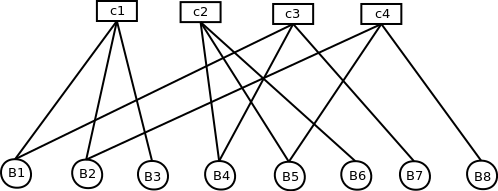
\includegraphics[height=3cm,width=6cm]{minSum1}
		\caption{ Tanner Graph }
	\end{figure}
	\end{column}%
\end{columns}
\end{frame}	
	

\begin{frame}[t]
\frametitle{ A priori initialization }  
\begin{columns}[totalwidth=\textwidth]
	\begin{column}{0.4\textwidth}
	\centering
	\begin{itemize}
	\item A priories are calculated by soft information of the code bits.	
	\item 	$
	\alert{aPriori[I] =}
	$
	$
	\alert{ -4 * C[I] * R * \dfrac{Eb}{No}}
	$ 
	\item where C[I] = $i^{th}$ code block
	\item R = code rate
	\item $\dfrac{Eb}{No}$ = signal to noise power ratio
	\end{itemize}
 
			
	\end{column}% 
	   		
	\begin{column}{0.6\textwidth}
	\centering
	\begin{figure}
	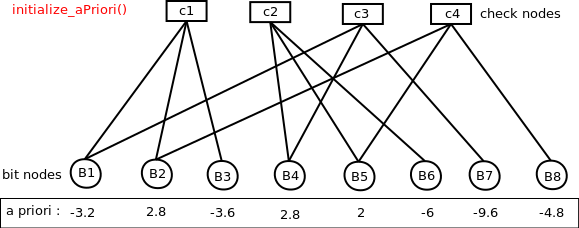
\includegraphics[height=4cm,width=7cm]{minSum2}
	\caption{ A priori initialization }
	\end{figure}
	\end{column}%
\end{columns}
\end{frame}



\begin{frame}[t]
\frametitle{ Message initialization }  
\begin{columns}[totalwidth=\textwidth]
	\begin{column}{0.4\textwidth}
	\centering
	\begin{itemize}
	\item Messages are the information propagating from bit nodes to check nodes.
	\item These are initialized to a priori of their respective bit node.	
	\item 	$ \alert{message[I][J] =} 
	$
	$
	\alert{aPriori[I]} 
	$ 
	\end{itemize}
 
			
	\end{column}% 
	   		
	\begin{column}{0.6\textwidth}
	\centering
	\begin{figure}
	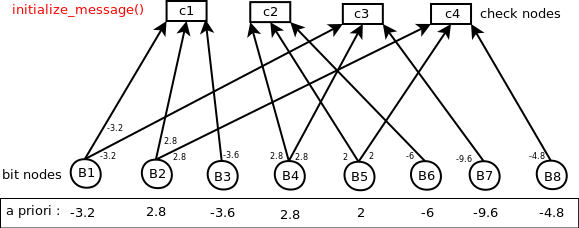
\includegraphics[height=4cm,width=7cm]{minSum3}
	\caption{ Message initialization }
	\end{figure}
	\end{column}%
\end{columns}
\end{frame}


\begin{frame}[t]
\frametitle{ Extrinsic information calculation }  
\vspace{-5mm}
\begin{columns}[totalwidth=\textwidth]
	\begin{column}{0.3\textwidth}
	\centering
	\begin{itemize}
	\item Extrinsic information of a bit node is calculated min sum of all the message's connected to 
	that particular check node. 	
	\end{itemize}
 
			
	\end{column}% 
	   		
	\begin{column}{0.7\textwidth}
	\centering
	\begin{figure}
	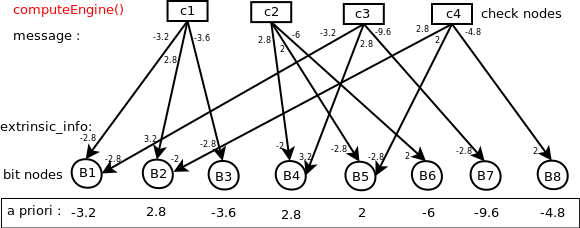
\includegraphics[height=4.5cm,width=8cm]{minSum4}
	\end{figure}
	\end{column}%
\end{columns}

\begin{itemize}

\item \alert{$|E_{(j,i)}| =  Min_{i'\in B_j \ i'\neq i }|M_{j,i'}|   $ }
\item \alert{$sign({E_{(j,i)}}) =  \prod_{i'\in B_j \ i'\neq i }sign(M_{j,i'})   $ }
\end{itemize}
\end{frame}


\begin{frame}[t]
\frametitle{ A posteriori calculation }  
\vspace{-5mm}
\begin{columns}[totalwidth=\textwidth]
	\begin{column}{0.3\textwidth}
	\centering
	\begin{itemize}
	\item A posteriori probabilities are the output bit probabilities.
	\item These are used to modify the code block after every iteration.
	\end{itemize}
 
			
	\end{column}% 
	   		
	\begin{column}{0.7\textwidth}
	\centering
	\begin{figure}
	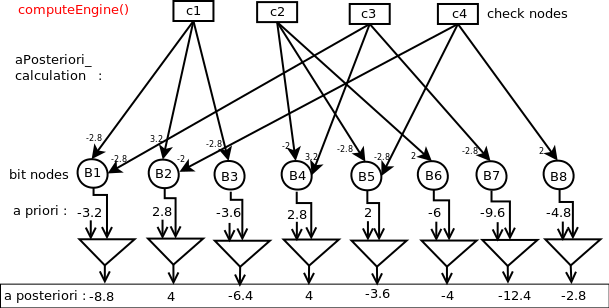
\includegraphics[height=4.5cm,width=8cm]{minSum5}
	\end{figure}
	\end{column}%
\end{columns}

\begin{itemize}

\item \alert{$ aPosteriori[I] = \sum_{j\in A_i} E_{j,i} + aPriori[I] $}
\end{itemize}
\end{frame}


\begin{frame}[t]
\frametitle{ isDecoded block }  
\vspace{-5mm}
\begin{columns}[totalwidth=\textwidth]
	\begin{column}{0.48\textwidth}
	\centering
	\begin{itemize}
	\item This block flips a bit if it is different form hard decision 
	of the a posteriori probability of the bit. Thus, modifies the code block.  
	\item If, no bit got flipped then decoding stops.
	\end{itemize}
 
			
	\end{column}% 
	   		
	\begin{column}{0.52\textwidth}
	\centering
	\begin{figure}
	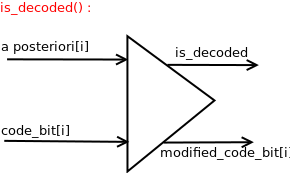
\includegraphics[height=3.5cm,width=5cm]{minSum6}
	\end{figure}
	\end{column}%
\end{columns}

\begin{itemize}

\item \alert{$ is\_decoded =  1$ ;\\
if $\forall$ i code\_bit[I] = hard\_decision(aPosteriori[I]) }
\end{itemize}
\end{frame}


\begin{frame}[t]
\frametitle{ Updating messages }  
\vspace{-5mm}
\begin{columns}[totalwidth=\textwidth]
	\begin{column}{0.3\textwidth}
	\centering
	\begin{itemize}
	\item Messages are updated and transmitted back to start the next iteration of decoding.
	\end{itemize}
 
			
	\end{column}% 
	   		
	\begin{column}{0.7\textwidth}
	\centering
	\begin{figure}
	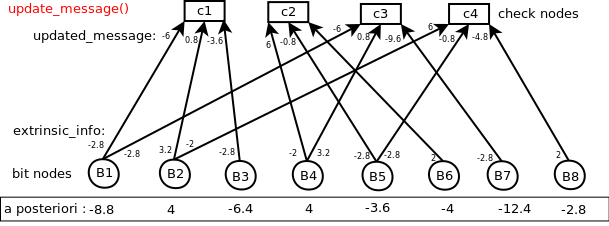
\includegraphics[height=5cm,width=8cm]{minSum7}
	\end{figure}
	\end{column}%
\end{columns}

\begin{itemize}

\item \alert{$   message_{(j,i)} = aPosteriori[i] - E_{(j,i)}  $}
\end{itemize}
\end{frame}





\begin{frame}[t]
\frametitle{  }                                 % and a label for
\alert{ minSumDecode()	: }
\begin{algorithmic}                   
    \STATE $initialize\_aPriori() $
    \STATE $initializeMessage() $
    \WHILE{$nitr \geq Max\_nitr$}    
    	\STATE$ initialize\_aPosteriori() \Leftarrow aPriori $
   		\STATE $initializeExtrinsicInfo() \Leftarrow 0 $
  		\STATE$\textbf{checkNodeComputeEngine()}$
    	\STATE $is\_decoded = checkIsDecode()$
    	\IF{$is\_decoded = 1$}
        	\STATE break 
    	\ELSE
        	\STATE $updateMessage()$
     	\ENDIF 
     $nitr++$       	
    \ENDWHILE 
\end{algorithmic}
\end{frame}

\begin{frame}[t]
\frametitle{  }  
\begin{figure}
       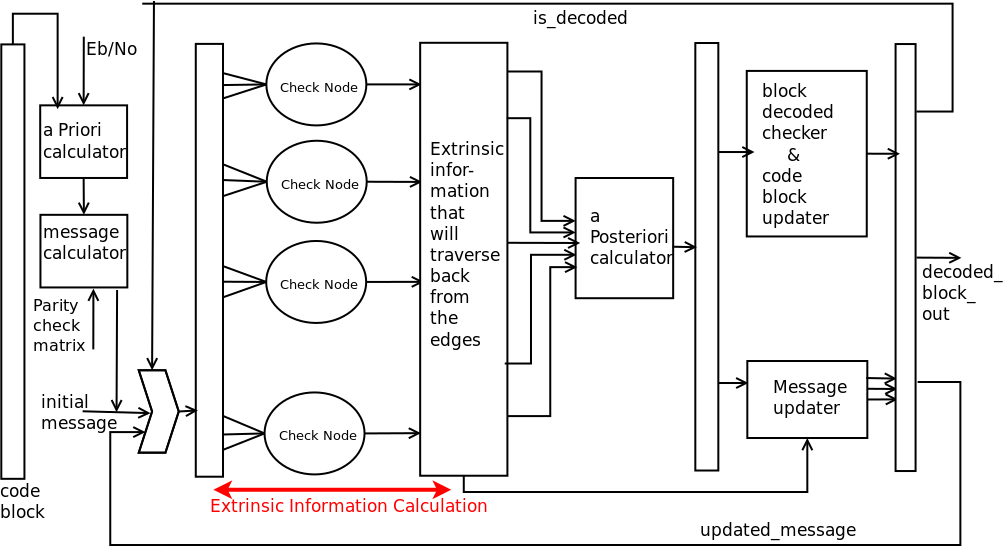
\includegraphics[height=7cm,width=11cm]{minSum}
       \end{figure}
\end{frame}

\begin{frame}[t]
\frametitle{ Algorithmic complexity at each stage }  
\begin{itemize}
\item A priori calculation	:	O(m) 
\item Message calculation 	:	O(m x p)
\item Extrinsic information calculation	: O(m x p x (p-1) ) $\approx $O($mp^{2}$)
\item A posteriori calculation : O(m x p)
\item Message updation : O(m x p)
\item block decoded calculation \& code block updation	: O(m)
\end{itemize}
\end{frame}


\section{Modified min sum algorithm}

\section{ Modified min sum algorithm}
\begin{frame}[t]
\frametitle{ Partitioning matrix  }  
\begin{itemize}
\item After partitioning the matrix we get four matrices as follows 	:
\[
H = \left[ \begin{array}{c|c}  
H11  & H12     \\ \hline
H21  & H22     \end{array} \right] 
\] 
\item example :
\[
\begingroup % keep the change local
\setlength\arraycolsep{1pt}
\left[ \begin{array} {c|cccccccc} 
  &    c1 &   c2 &   c3 &  c4  &  c5  &  c6  &  c7  &  c8 \\ \hline
r1 &    1  &   1  &   1  &   0  &   0  &   0  &   0  &   0 \\
r2 &    0  &   0  &   0  &   1  &   1  &   1  &   0  &   0 \\ 
r3 &    1  &   0  &   0  &   1  &   0  &   0  &   1  &   0 \\
r4 &    0  &   1  &   0  &   0  &   1  &   0  &   0  &   1 \end{array} \right] 
     \Rightarrow
\left[ \begin{array} {c|cccc|cccc} 
  &    c4 &   c6 &   c7 &  c1  &  c2  &  c3  &  c8  &  c5 \\ \hline  
r2 &     1  &   1  &   0  &   0  &   0  &   0  &   0  &   1 \\
r3 &     1  &   0  &   1  &   1  &   0  &   0  &   0  &   0 \\ \hline
r1 &     0  &   0  &   0  &   1  &   1  &   1  &   0  &   0 \\
r4 &     0  &   0  &   0  &   0  &   1  &   0  &   1  &   1 \end{array} \right] 
\endgroup
\]
\item H12 and H21 are highly sparse.
\end{itemize}
\end{frame}







\begin{frame}[t]
\frametitle{ Modified min sum algorithm }                                 % and a label for
\alert{ main.c }
\begin{algorithmic}                   
    \REQUIRE Parity check matrix in row compressed form.
    \STATE readMatrixH11()
    \STATE readMatrixH12()
    \STATE readMatrixH21()
    \STATE readMatrixH22()
    \STATE readCodeBlock1()
    \STATE readCodeBlock2()
    \STATE \textbf{modifiedMinSumDecode()}
    \STATE findAccuracy()

\end{algorithmic}
\end{frame}

\begin{frame}[t]
\frametitle{ A priori initialization }  
\begin{columns}[totalwidth=\textwidth]
	\begin{column}{0.4\textwidth}
	\centering
	\begin{itemize}
	\item A priories are calculated by soft information of the code bits.	
	\item 	$
	\alert{aPriori[I] =}
	$
	$
	\alert{ -4 * C[I] * R * \dfrac{Eb}{No}}
	$ 
	\item where C[I] = $i^{th}$ code block
	\item R = code rate
	\item $\dfrac{Eb}{No}$ = signal to noise power ratio
	\end{itemize}
 
			
	\end{column}% 
	   		
	\begin{column}{0.6\textwidth}
	\centering
	\begin{figure}
	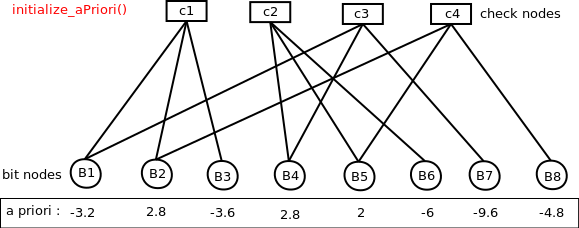
\includegraphics[height=4cm,width=7cm]{minSum2}
	\caption{ A priori initialization }
	\end{figure}
	\end{column}%
\end{columns}
\end{frame}


\begin{frame}[t]
\frametitle{ A priori initialization }  
\vspace{-5mm}
\begin{figure}
       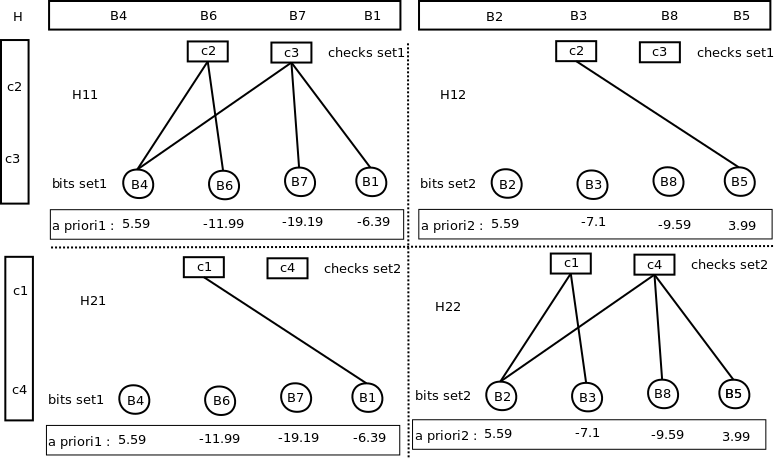
\includegraphics[height=7cm,width=11cm]{minSumModified1}
       \end{figure}
\end{frame}


\begin{frame}[t]
\frametitle{ Message initialization }  
\begin{columns}[totalwidth=\textwidth]
	\begin{column}{0.4\textwidth}
	\centering
	\begin{itemize}
	\item Messages are the information propagating from bit nodes to check nodes.
	\item These are initialized to a priori of their respective bit node.	
	\item 	$ \alert{message[I][J] =} 
	$
	$
	\alert{aPriori[I]} 
	$ 
	\end{itemize}
 
			
	\end{column}% 
	   		
	\begin{column}{0.6\textwidth}
	\centering
	\begin{figure}
	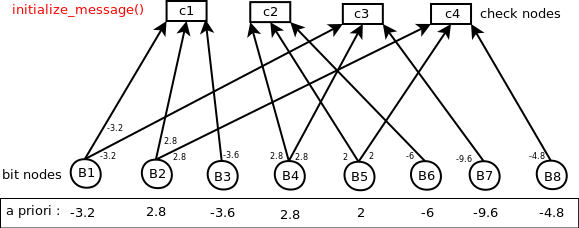
\includegraphics[height=4cm,width=7cm]{minSum3}
	\caption{ Message initialization }
	\end{figure}
	\end{column}%
\end{columns}
\end{frame}


\begin{frame}[t]
\frametitle{ Message initialization }  
\vspace{-5mm}
\begin{figure}
       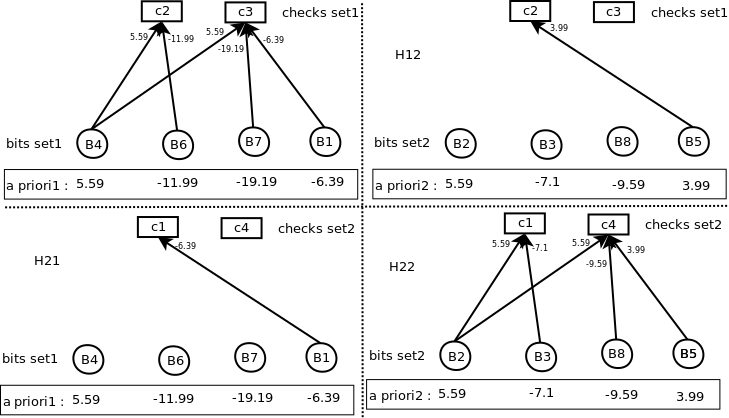
\includegraphics[height=7cm,width=11cm]{minSumModified2}
       \end{figure}
\end{frame}


\begin{frame}[t]
\frametitle{ Extrinsic information calculation }  
\vspace{-5mm}
\begin{columns}[totalwidth=\textwidth]
	\begin{column}{0.3\textwidth}
	\centering
	\begin{itemize}
	\item Extrinsic information of a bit node is calculated min sum of all the message's connected to 
	that particular check node. 	
	\end{itemize}
 
			
	\end{column}% 
	   		
	\begin{column}{0.7\textwidth}
	\centering
	\begin{figure}
	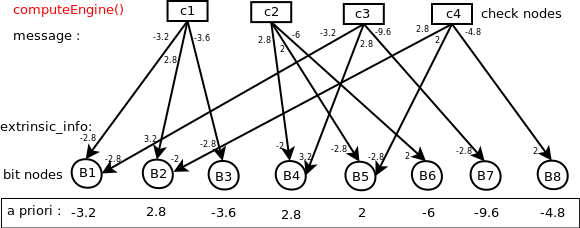
\includegraphics[height=4.5cm,width=8cm]{minSum4}
	\end{figure}
	\end{column}%
\end{columns}

\begin{itemize}

\item \alert{$|E_{(j,i)}| =  Min_{i'\in B_j \ i'\neq i }|M_{j,i'}|   $ }
\item \alert{$sign({E_{(j,i)}}) =  \prod_{i'\in B_j \ i'\neq i }sign(M_{j,i'})   $ }
\end{itemize}
\end{frame}

\begin{frame}[t]
\frametitle{ Partial Extrinsic information calculation }  
\vspace{-5mm}
\begin{figure}
       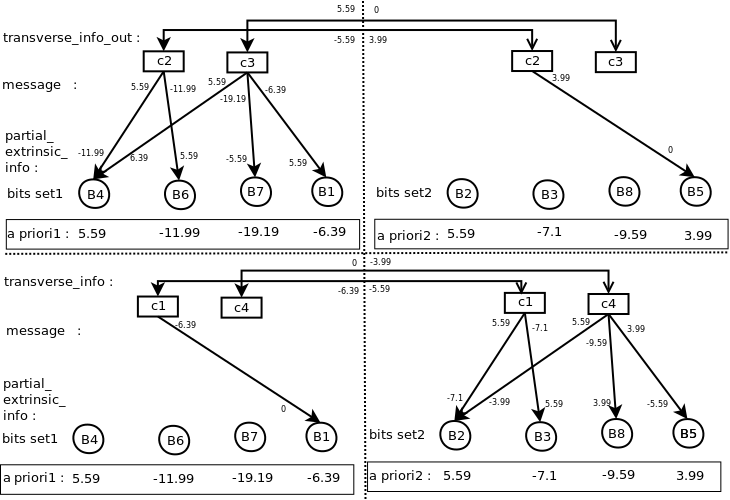
\includegraphics[height=7cm,width=11cm]{minSumModified3}
       \end{figure}
\end{frame}

\begin{frame}[t]
\frametitle{ Update extrinsic information }  
\vspace{-5mm}
\begin{figure}
       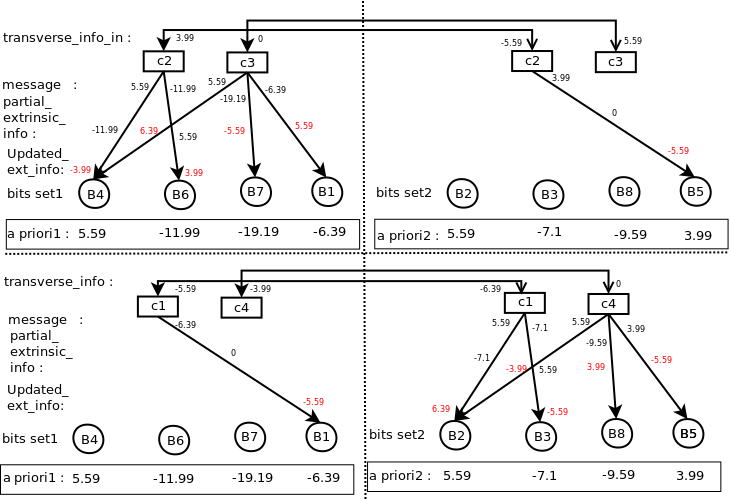
\includegraphics[height=7cm,width=11cm]{minSumModified4}
       \end{figure}
\end{frame}

\begin{frame}[t]
\frametitle{  }                                 % and a label for
\alert{ modifiedMinSumDecode()	: }
\begin{algorithmic}                   
    \STATE $initialize\_aPriori(aPriori1) $
    \STATE $initialize\_aPriori(aPriori2) $
    \STATE $initializeMessage(message11) $
    \STATE $initializeMessage(message12) $
    \STATE $initializeMessage(message21) $
    \STATE $initializeMessage(message22) $
    \WHILE{$nitr \geq Max\_nitr$}    
    	\STATE$ initialize\_aPosteriori(aPosteriori1) \Leftarrow aPriori1 $
    	\STATE$ initialize\_aPosteriori(aPosteriori2) \Leftarrow aPriori2 $
   		\STATE $initializeExtrinsicInfo(ext\_info11) \Leftarrow 0 $
   		\STATE $initializeExtrinsicInfo(ext\_info12) \Leftarrow 0 $
   		\STATE $initializeExtrinsicInfo(ext\_info21) \Leftarrow 0 $
   		\STATE $initializeExtrinsicInfo(ext\_info22) \Leftarrow 0 $
   		\STATE ... 		
   		 \ENDWHILE 
\end{algorithmic}
\end{frame}

\begin{frame}[t]
\frametitle{  }                                 % and a label for
\alert{ modifiedMinSumDecode()	: }
\begin{algorithmic}   
\WHILE{...} 
\STATE ...               
\STATE$computeEngine(H11,message11,ext\_info11,trans\_info11\_12)$
\STATE$computeEngine(H22,message22,ext\_info22,trans\_info22\_12)$
\STATE$computeEngine(H12,message12,ext\_info12,trans\_info12\_11)$
\STATE$computeEngine(H21,message21,ext\_info21,trans\_info21\_22)$
\STATE$transverseCorrection(H11,transverse\_info12\_11,ext\_info11)$
\STATE$transverseCorrection(H22,transverse\_info21\_22,ext\_info22)$
\STATE$transverseCorrection(H21,transverse\_info22\_21,ext\_info21)$
\STATE$transverseCorrection(H12,transverse\_info11\_12,ext\_info12)$
\STATE$update\_aPosteriori (H11 , ext\_info11 ,aPosteriori1)$
\STATE$update\_aPosteriori (H22 , ext\_info22 ,aPosteriori2)$
\STATE$update\_aPosteriori (H12 , ext\_info12 ,aPosteriori1)$
\STATE$update\_aPosteriori (H21 , ext\_info21 ,aPosteriori2)$
\STATE ...
     	
 \ENDWHILE    


  		
\end{algorithmic}
\end{frame}


\begin{frame}[t]
\frametitle{  }                                 % and a label for
\alert{ modifiedMinSumDecode()	: }
\begin{algorithmic}   
\WHILE{...} 
\STATE ...  
\STATE$is\_decoded1 = checkIsdecoded( code\_block1 , aPosteriori1 ) $
\STATE$is\_decoded2 = checkIsdecoded( code\_block2 , aPosteriori2 ) $              
		\IF{$(is\_decoded1 \&\& is\_decoded2)== 1$}
        	\STATE break 
    	\ELSE
        	\STATE $updateMessage(ext\_info11 ,aPosteriori1 ,message11)$
        	\STATE $updateMessage(ext\_info22 ,aPosteriori2 ,message22)$
        	\STATE $updateMessage(ext\_info12 ,aPosteriori1 ,message12)$
        	\STATE $updateMessage(ext\_info21 ,aPosteriori2 ,message21)$
     	\ENDIF 
\STATE $nitr++$  
 \ENDWHILE    


  		
\end{algorithmic}
\end{frame}

\begin{frame}[t]
\frametitle{  }  
\begin{figure}
       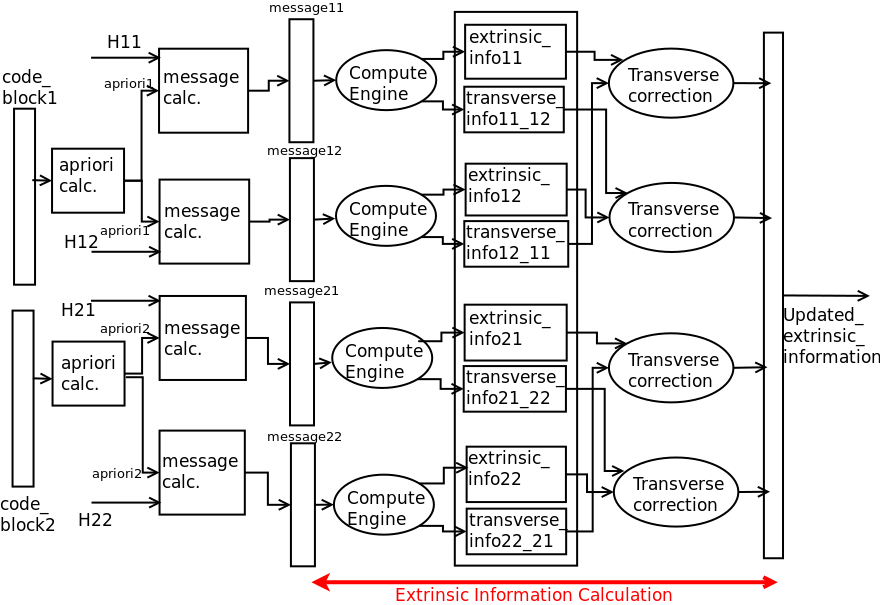
\includegraphics[height=7cm,width=11cm]{minSumModified}
       \end{figure}
\end{frame}

\begin{frame}[t]
\frametitle{ State Diagram }  
\begin{figure}
       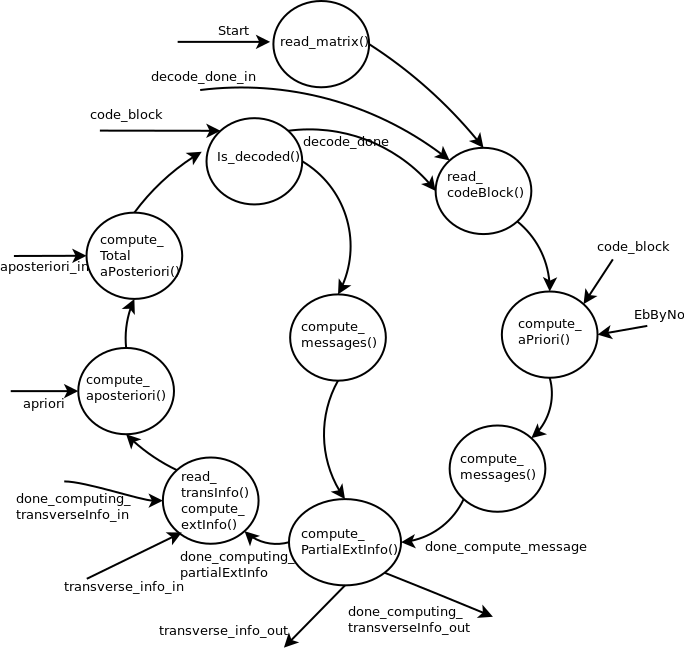
\includegraphics[height=7cm,width=8cm]{stateDiagram}
       \end{figure}
\end{frame}


\begin{frame}[t]
\frametitle{ Matrix Initialization }  
\begin{itemize}
\item Maximum file length till matrix order 12k is $\approx$ 60k, thus we have to store 60k values of type uint16\_t.
\item thus taking 4 memory of 20k each .\\
 $uint16\_t \ mem[20,000]$
\item populate it with reading a pipe of size 64bits.
\item Thus writing 4 word at a time.
\item $\approx (60k/4)/4 $ clocks to write matrix in memory.
\end{itemize}
\end{frame}

\begin{frame}[t]
\frametitle{ Code block input }  
\begin{itemize}
\item Code block file length till matrix order 12k is $\approx$13k, thus we have to store $\approx$13k values of bit data type.
\item We can choose a thick pipe width of 256 bits or 512 bits. Thus it will take upto 64 or 32 clock cycles respectively to input a code block.
\end{itemize}
\end{frame}

%-----------------------------last slide------------------------------
%---------------------------end of document---------------------------

\end{document}